\documentclass[a4paper]{report}
\usepackage[english]{babel}
\usepackage{amsmath}
\usepackage{graphicx}
\usepackage{epstopdf}
\usepackage{enumerate}
\usepackage{pdfpages}
\usepackage{listings}
\usepackage{framed}
\title{Computer Networks: Network simulation}
\author{Jona Beysens (r0296825) \& Arnout Devos (r0305883)}

\newcommand{\opgave}[1]{\section{Question #1}}


\begin{document}
\maketitle
\chapter*{Exercise 1}

\section*{Question 1}
Figure~\ref{ex1:question1} shows the throughput at node 1 of the KotNet topology. 
In the beginning of the TCP transfer the slow start is observed. The rate at which the packets are received at node 1 converges to a constant value of around 500kbytes/s which equals the maximum download speed of 4Mbit/s. The little hills on top of the download rate can be explained by the inaccuracy of the perl visualization script.
\begin{figure}[h]
\centerline{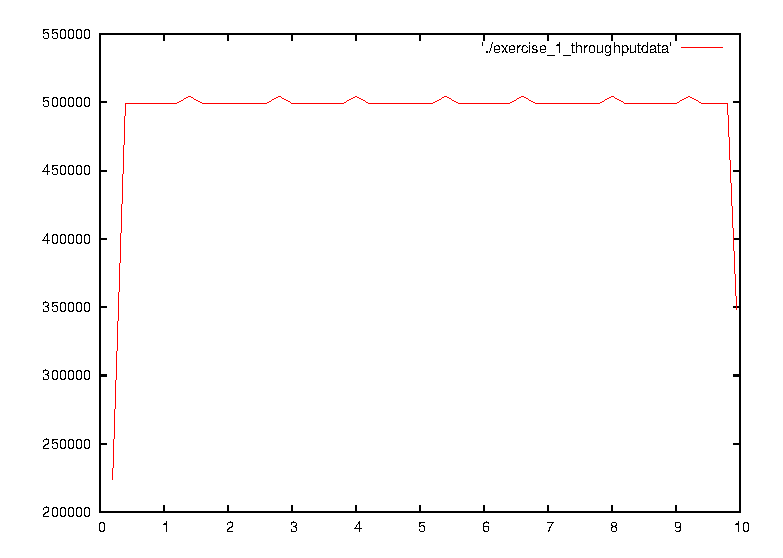
\includegraphics{pictures/E1Q1.eps}}
\caption{Throughput of FTP connection at node 1 of KotNet topology}
\label{ex1:question1}
\end{figure}

\section*{Question 2}
In the beginning of the TCP transfer the slow start occurs. When the UDP transmission kicks in, a significant drop in TCP throughput is observed. This is caused by the upload bandwidth limitation of the cable modem: TCP sends an accumulated acknowledgements for received packets but the upload line is congested with UDP traffic as can be seen on the figure~\ref{ex1:question2}. Therefor, TCP throughput drops. Acknowledgements are lost due to the overloaded buffer. When the UDP traffic stops, the upload line isn't congested anymore and the slow start mechanism of TCP kicks in again. The throughput converges to the original value of 500kbytes/s.
\begin{figure}[h]
\centerline{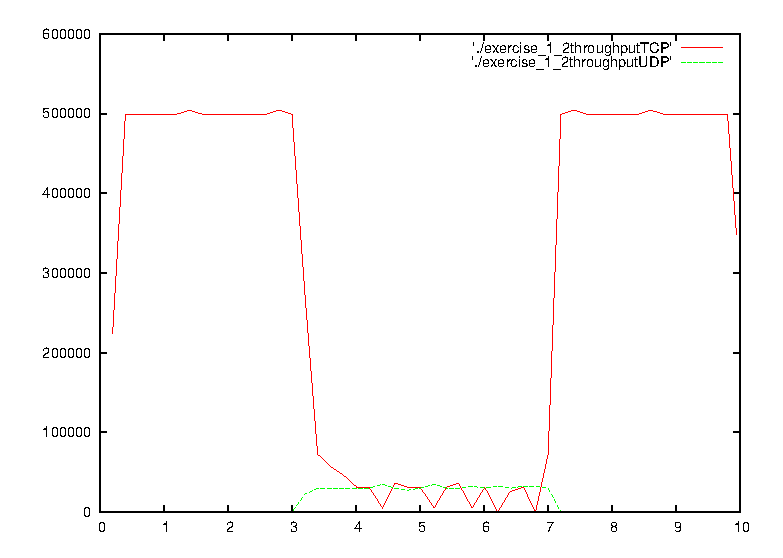
\includegraphics{pictures/E1Q2.eps}}
\caption{Throughput of FTP and CBR connection at node 1 of KotNet topology}
\label{ex1:question2}
\end{figure}

\section*{Question 3}
The CBR connection won't take the needed upload bandwidth for the acknowledgements of the TCP connection. 
If the assigned bandwidth for TCP is large enough to transfer the acknowledgements without congesting the buffer, the TCP throughput will sustain its maximum value. The UDP throughput will adapt to the assigned bandwidth.  

\section*{Question 4}
If we take the case where the 100 Mbit uplinks and downlinks are preserved, the traffic will be even more distorted. Because a bigger packet loss rate occurs at the buffers, even more TCP acknowledgements will be discarded which results in a lower TCP throughput. UDP throughput also drops to approximately 100kbits/s as the upload line is congested with UDP traffic.

\section*{Question 5}
The TCP throughput doesn't drop that much as the situation where the rate of sending UDP packets isn't limited to 30kbytes/s (see figure~\ref{ex1:question5}). Although TCP experiences some jitter as it needs a higher bandwidth to transmit all its acknowledgements immediately. A possible solution to this jitter would be to increase TCP packet size and by this reduce the acknowledgement rate which leads to a maximum use of the 4 Mbit bandwidth.
\begin{figure}[h]
\centerline{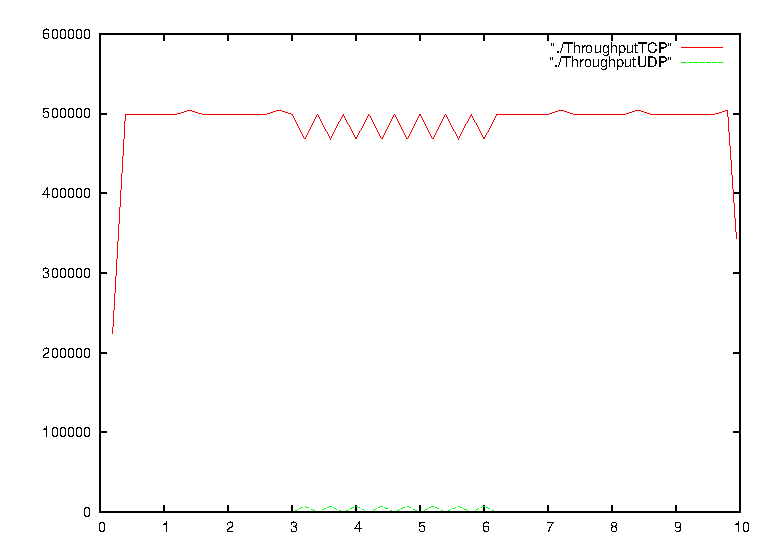
\includegraphics{pictures/E1Q5.eps}}
\caption{Throughput of FTP and CBR connection at node 1 of KotNet topology with limited upload bandwith of CBR connection}
\label{ex1:question5}
\end{figure}

\section*{Question 6}
\begin{enumerate}[a)]
\item
With 10 users, the amount of users and bandwidth scale with the same factor, so the performance will be the same.
When there are only 5 users using the network, one can reach a better performance. Suppose that the UDP traffic also increases by the same factor. The TCP traffic will then have twice as much bandwidth available.
\item
Yes, the performance will be more oscillating because the available bandwidth on the network varies randomly. Other users will suffer when one user decides to have a lot of UDP traffic because this UDP traffic obstructs acknowledgements from the TCP traffic which results in congestion. The buffers will be overloaded and time-outs will occur.
\end{enumerate}

\chapter*{Exercise 2}

\section*{Question 1}
From figure~\ref{ex2:question1} we can see that when the web traffic bursts start at 5.0s, the long lasting FTP application does not immediately experience a drop in throughput. This is due to the slow start mechanism of the TCP connection which only reaches the maximum throughput at around 6.0s. The burst of HTTP requests will cause congestion. This results in reduced throughput and retransmission of dropped packets. We can see this on the graph where the burst traffic lasts until 8.0s instead of 7.0s. The bursts of HTTP traffic beginning at 10.0s and 15.0s can be analyzed analogously.
\begin{figure}[h]
\centerline{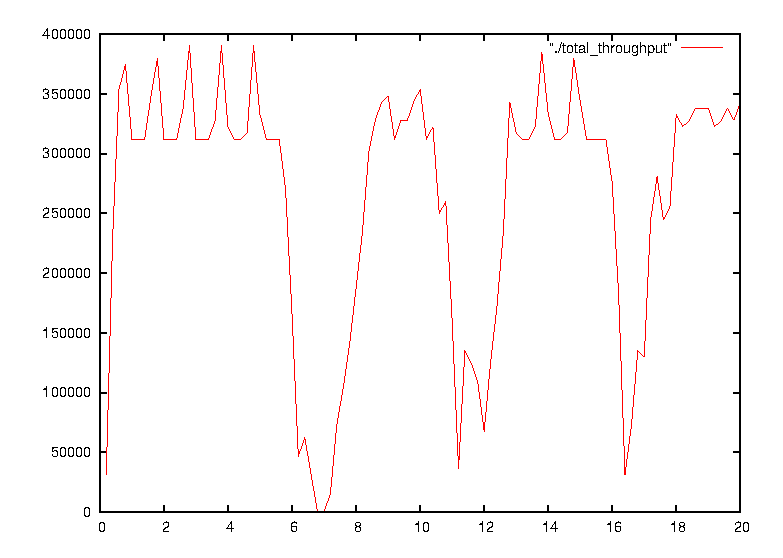
\includegraphics{pictures/E2Q1.eps}}
\caption{Throughput of FTP connection at node 2 of topology of exercise 2}
\label{ex2:question1}
\end{figure}

\section*{Question 2}
The different phases of the TCP algorithm are the slow start phase and the congestion avoidance phase in which the window size grows exponentially and linearly respectively. We can see this on figure~\ref{ex2:question2}: the algorithm begins in the slow start phase. The window size grows exponentially. When the window size equals the slow start threshold, a nearly linearly increasing windows size is observed. The TCP algorith is now in the congestion avoidance phase. When congestion occurs and is detected, the window size will drop and the algorithm will start over again. A new threshold will be calculated when congestion occurs. The value of this new threshold is equal to half the value of the current slow start threshold.
\begin{figure}[h]
\centerline{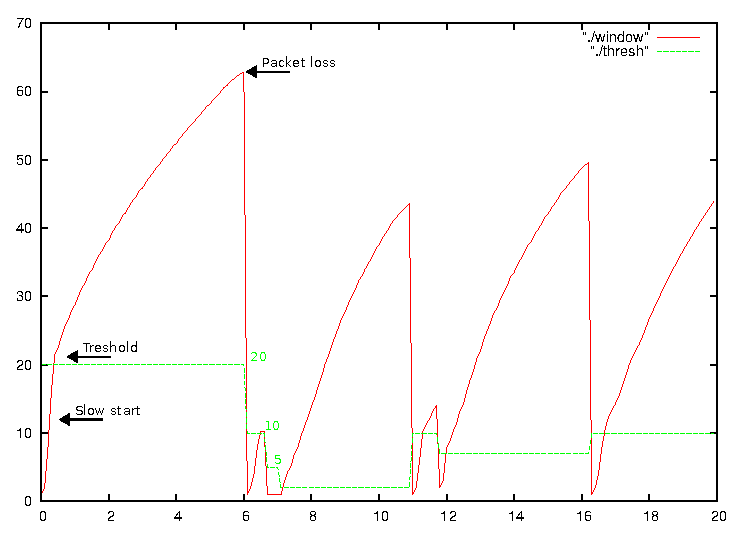
\includegraphics{pictures/E2Q2Marked.eps}}
\caption{Congestion window size and slow start threshold of main FTP application with TCP Tahoe}
\label{ex2:question2}
\end{figure}

\section*{Question 3}
The \textit{additive increase/multiple decrease (AIMD)} algorithm is used in TCP to make a feedback loop based on congestion signals. As congestion is a bad thing to happen because it also influences other clients on the network, a rapid decrease in traffic is needed to minimize the effect of the congestion. This is done by multiple decrease whereas when the network is not congested one can slowly increase the traffic with additive increase. It is shown by \textbf{Chiu et al}\footnote{Chiu, Dah-Ming; Raj Jain (1989)."Analysis of increase and decrease algorithms for congestion avoidance in computer networks". Computer Networks and ISDN systems 17:1-14.} that this asymmetry in buildup and break down speeds results in convergence to an optimal point.

A few reasonable values for the congestion window are shown on figure~\ref{ex2:question2}.
The first interval where the TCP congestion avoidance algorithm is active is [0.45 – 5.45] as can be seen on the graph.

\section*{Question 4}
The difference between Tahoe and Reno lies in the fact that when congestion occurs, Tahoe always reduces the window size to 1 whereas Reno will perform fast recovery. This fast recovery will ensure that after 3 received duplicate acknowledgements the packet has not been transmitted succesfully. The congestion window size will be halved instead of lowered to 1 as with Tahoe. When more than one packet is lost and fast retransmission does not recover adequately, Reno acts the same way as Tahoe: the congestion window size will drop to 1 and slow start occurs. This happens most of the time as can be seen on figure~\ref{ex2:question4}.
\begin{figure}[h]
\centerline{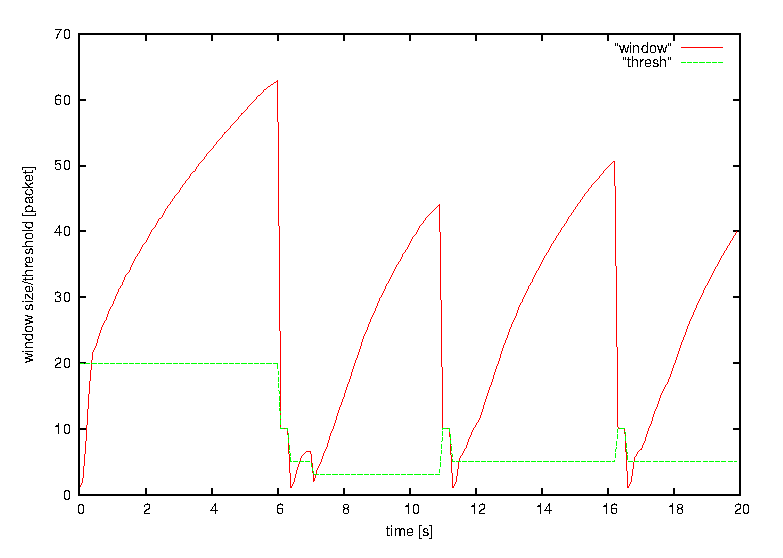
\includegraphics{pictures/E2Q4.eps}}
\caption{Congestion window size and slow start threshold of main FTP application with TCP Reno}
\label{ex2:question4}
\end{figure}
\end{document}

